\section*{Anexo A. Recolección de la información}
\addcontentsline{toc}{section}{Anexo A. Recolección de la información}

	\subsection*{Encuesta}
	\addcontentsline{toc}{subsection}{Encuesta}
	
	{Para obtener la información base para el desarrollo del proyecto, fue indispensable utilizar la técnica de recolección de información “encuesta”, donde se plasmaron las inquietudes que permitieron estructurar adecuadamente el proyecto.\\
		
	Las encuestas realizadas fueron las siguientes (se utilizó la plataforma Formularios de Google para publicar y obtener los resultados de estas):
	
	
		\subsubsection*{Encuesta 1 - Viabilidad}
		\addcontentsline{toc}{subsubsection}{Encuesta 1 - Viabilidad}
		
			\begin{enumerate}
				
				\item ¿Ha recurrido el sistema de “fiado” que utilizan algunos tenderos para adquirir productos?
				
					\begin{enumerate}
						\item Si.
						\item No.
					\end{enumerate}
				
				\item ¿Ha tenido problemas al momento de pagar sus productos fiados, ya que el monto de la deuda es mayor o menor al que tenía en mente?
				
					\begin{enumerate}
						\item Si.
						\item No.
					\end{enumerate}	
				
				\item Cuándo realiza un préstamo, ¿dónde realiza el registro de este, para su posterior control?
					
					\begin{enumerate}
						\item Tomo notas en el celular.
						\item Tomo notas en cuadernos o agendas.
						\item No tomo notas.
						\item Otro.
					\end{enumerate}
				
				\item ¿Suele olvidarse de las deudas que tienen algunas personas con usted (personas de confianza)?
				
					\begin{enumerate}
						\item Si.
						\item No.
					\end{enumerate}	
				
				\item Considera que utilizar una plataforma Web que permita gestionar los fiados y prestamos es:
				
					\begin{enumerate}
						\item Pertinente.
						\item Innecesaria.
					\end{enumerate}
				
			\end{enumerate}
		
		\subsubsection*{Tabulación encuesta 1}
		\addcontentsline{toc}{subsubsection}{Tabulación encuesta 1}
		{Para esta encuesta, se alcanzaron a encuestar 71 personas que contestaron lo siguiente:
		
		\begin{figure}[H]
			\centering
			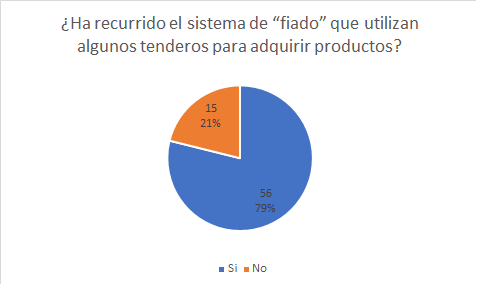
\includegraphics[width=0.8\linewidth]{annexes/e1-p1.png}
			\caption{Diagrama de torta E-1 P-1}
		\end{figure}
	
		\begin{figure}[H]
			\centering
			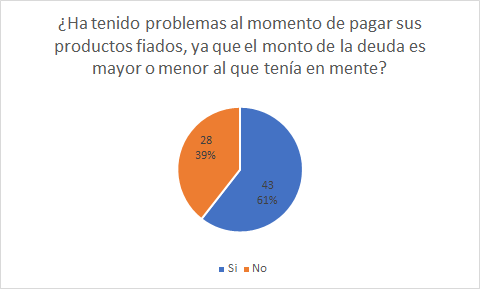
\includegraphics[width=0.8\linewidth]{annexes/e1-p2.png}
			\caption{Diagrama de torta E-1 P-2}
		\end{figure}
	
		\begin{figure}[H]
			\centering
			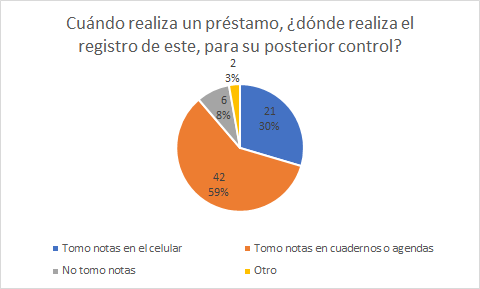
\includegraphics[width=0.8\linewidth]{annexes/e1-p3.png}
			\caption{Diagrama de torta E-1 P-3}
		\end{figure}
	
		\begin{figure}[H]
			\centering
			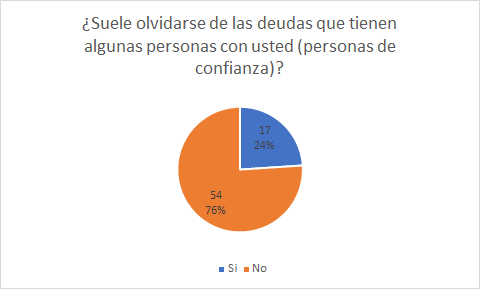
\includegraphics[width=0.8\linewidth]{annexes/e1-p4.png}
			\caption{Diagrama de torta E-1 P-4}
		\end{figure}
	
		\begin{figure}[H]
			\centering
			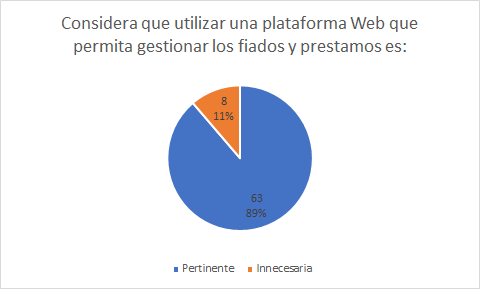
\includegraphics[width=0.8\linewidth]{annexes/e1-p5.png}
			\caption{Diagrama de torta E-1 P-5}
		\end{figure}
		}
		
		\subsubsection*{Encuesta 2 - Satisfacción del proyecto}
		\addcontentsline{toc}{subsubsection}{Encuesta 2 - Satisfacción del proyecto}
		
			\begin{enumerate}
				
				\item Utilizando Tru\$tMe como tendero sus ventas han:
				
				\begin{enumerate}
					\item Aumentado.
					\item Se mantuvieron.
					\item Disminuido.
				\end{enumerate}
				
				\item Utilizando Tru\$tMe como consumidor, ¿Ha tenido dudas con respecto a los pagos a realizar?
				
				\begin{enumerate}
					\item Si.
					\item No.
				\end{enumerate}	
				
				\item ¿Le permite Tru\$tMe tener un mejor control de sus finanzas visualizando sus deudas y prestamos actuales?
				
				\begin{enumerate}
					\item Si.
					\item No.
				\end{enumerate}
				
			\end{enumerate}
		
		\subsubsection*{Tabulación encuesta 2}
		\addcontentsline{toc}{subsubsection}{Tabulación encuesta 2}
		
		{Para esta encuesta, se alcanzaron a encuestar 23 personas que contestaron lo siguiente:
			
			\begin{figure}[H]
				\centering
				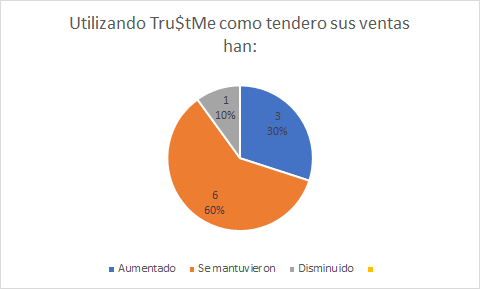
\includegraphics[width=0.8\linewidth]{annexes/e2-p1.png}
				\caption{Diagrama de torta E-2 P-1}
			\end{figure}
			
			\begin{figure}[H]
				\centering
				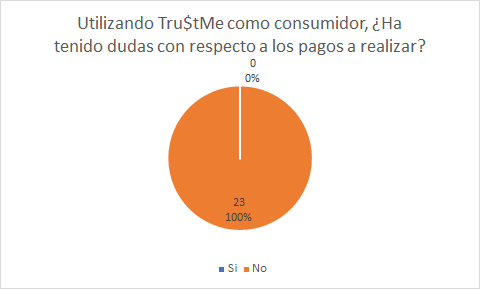
\includegraphics[width=0.8\linewidth]{annexes/e2-p2.png}
				\caption{Diagrama de torta E-2 P-2}
			\end{figure}
			
			\begin{figure}[H]
				\centering
				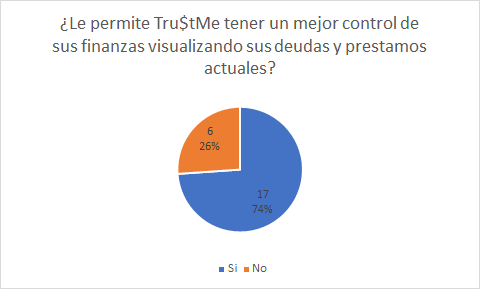
\includegraphics[width=0.8\linewidth]{annexes/e2-p3.png}
				\caption{Diagrama de torta E-2 P-3}
			\end{figure}
		}
		
	}
	

	